%\documentclass[handout]{beamer}
\documentclass{beamer}

\mode<presentation>
{
%\usetheme{Singapore}
%\usetheme{Warsaw}
\usetheme{Malmoe}
\useinnertheme{circles}
\useoutertheme{infolines}
% \useinnertheme{rounded}

\setbeamercovered{transparent}
}

\usepackage[english]{babel}
\usepackage[latin1]{inputenc}
\usepackage{bm,textpos,alltt,listings,multirow,ulem}

% font definitions, try \usepackage{ae} instead of the following
% three lines if you don't like this look
\usepackage{mathptmx}
\usepackage[scaled=.90]{helvet}
\usepackage{courier}
\usepackage[T1]{fontenc}
\usepackage{tikz}
\usetikzlibrary[shapes.arrows,arrows,shapes.misc]

% \usepackage{pgfpages}
% \pgfpagesuselayout{4 on 1}[a4paper,landscape,border shrink=5mm]

\usepackage{slashbox,multirow,listings,booktabs}
\usepackage{xspace}
\makeatletter
\DeclareRobustCommand\onedot{\futurelet\@let@token\@onedot}
\def\@onedot{\ifx\@let@token.\else.\null\fi\xspace}
\def\eg{{e.g}\onedot} \def\Eg{{E.g}\onedot}
\def\ie{{i.e}\onedot} \def\Ie{{I.e}\onedot}
\def\cf{{c.f}\onedot} \def\Cf{{C.f}\onedot}
\def\etc{{etc}\onedot}
\def\vs{{vs}\onedot}
\def\wrt{w.r.t\onedot}
\def\dof{d.o.f\onedot}
\def\etal{{et al}\onedot}
\makeatother

\usepackage{tikz}
\usetikzlibrary[shapes,shapes.arrows,arrows,shapes.misc,fit,positioning]

\usepackage{siunitx}
\DeclareSIUnit\year{a}
\DeclareSIUnit\byte{B}
\sisetup{retain-unity-mantissa = false}

\usepackage{fancyvrb}
\usepackage{minted}
\newminted{c}{gobble=2}
\newminted{python}{gobble=2}
%\newmint[cverb]{c}{} 
\newcommand\cverb[1][]{\SaveVerb[%
    aftersave={\textnormal{\UseVerb[#1]{vsave}}}]{vsave}}
\newcommand\cfunc[1][]{\SaveVerb[%
    aftersave={\textnormal{\UseVerb[#1]{vsave}\texttt{()}}}]{vsave}}
\newcommand\pyverb[1][]{\SaveVerb[%
    aftersave={\textnormal{\UseVerb[#1]{vsave}}}]{vsave}}
\def\asm#1{{\tt #1}}
\def\code#1{{\tt #1}}
\def\shell#1{{\tt \$ #1}}

\newcommand\email[1]{{\href{mailto:#1}{\nolinkurl{#1}}}}

\newcommand{\II}{\mathcal{I}}
\newcommand{\C}{\mathbb{C}}
\newcommand{\D}{\mathcal{D}}
\newcommand{\EE}{\mathcal{E}}
\newcommand{\F}{\mathcal{F}}
\newcommand{\I}{\mathcal{I}}
\newcommand{\N}{\mathcal{N}}
\newcommand{\PP}{\mathcal{P}}
\newcommand\Ppc{\ensuremath{\mathsf P}}
\newcommand{\bigO}{\ensuremath{\mathcal{O}}}
\newcommand{\R}{\mathbb{R}}
\newcommand{\Rz}{\mathcal{R}}
\newcommand{\QQ}{\mathcal Q}
\newcommand{\VV}{\mathcal V}
\newcommand{\ASM}{\mathrm{ASM}}
\newcommand{\RASM}{\mathrm{RASM}}

\newcommand{\kb}{\tt}
\newcommand{\Pk}[1]{\ensuremath{P_{#1}}}
\newcommand{\Qk}[1]{\ensuremath{Q_{#1}}}
\newcommand{\Pkdisc}[1]{\ensuremath{P_{#1}^{\text{disc}}}}
\newcommand{\Qkdisc}[1]{\ensuremath{Q_{#1}^{\text{disc}}}}
\newcommand{\blue}{\textcolor{blue}}
\newcommand{\green}{\textcolor{green!70!black}}
\newcommand{\red}{\textcolor{red}}
\newcommand{\brown}{\textcolor{brown}}
\newcommand{\cyan}{\textcolor{cyan}}
\newcommand{\magenta}{\textcolor{magenta}}
\newcommand{\yellow}{\textcolor{yellow}}
\newcommand{\mini}{\mathop{\rm minimize}}
\newcommand{\st}{\mbox{subject to }}
\newcommand{\lap}{\Delta}
\newcommand{\grad}{\nabla}
\newcommand\mtab{\hspace{\stretch{1}}}
\newcommand\ud{\,\mathrm{d}}
\newcommand\bslash{{$\backslash$}}
\newcommand\half{{\frac 1 2}}
\newcommand{\abs}[1]{\left\lvert #1 \right\rvert}
\newcommand{\bigabs}[1]{\big\lvert #1 \big\rvert}
\newcommand{\norm}[1]{\left\lVert #1 \right\rVert}
\newcommand\oneitem[1]{\begin{itemize} \item #1 \end{itemize}}
\newcommand\pfrak{{\mathfrak p}}
\newcommand\nfrak{{\mathfrak n}}
\newcommand\ff{\bm f}
\newcommand\mm{\bm m}
\newcommand\nn{\bm n}
\newcommand\uu{\bm u}
\newcommand\vv{\bm v}
\newcommand\ww{\bm w}
\newcommand\DD{D}
\newcommand{\tcolon}{\!:\!}
\DeclareMathOperator{\sgn}{sgn}
\DeclareMathOperator{\card}{card}
\DeclareMathOperator{\trace}{tr}
\DeclareMathOperator{\erf}{erf}
\DeclareMathOperator{\sspan}{span}
\renewcommand{\bar}{\overline}
% \DeclareMathOperator{\divergence}{div}
% \renewcommand\div\divergence
\renewcommand{\div}{{\nabla \cdot}}
\newcommand\spliceop{\leftrightsquigarrow}
\newcommand\splice[5]{{#1} \overset{#5}{\underset{#3,#4}{\leftrightsquigarrow}} {#2}}
\newcommand{\ip}[2]{{\left\langle #1, #2 \right\rangle}}
\newcommand{\Linfty}{{L^\infty}}

% Dimensionless numbers
\newcommand{\Peclet}{{\mathrm{Pe}}}
\newcommand{\Reynolds}{{\mathrm{Re}}}
\newcommand{\Rayleigh}{{\mathrm{Ra}}}
\newcommand{\Mach}{{\mathrm{Ma}}}
\newcommand{\Prandtl}{{\mathrm{Pr}}}
\newcommand{\Grashof}{{\mathrm{Gr}}}

\newcommand{\PETSc}{{PETSc}}
\newcommand{\Dohp}{{Dohp}}
\newcommand\libmesh{\texttt{libMesh}}
\newcommand\dealii{\texttt{Deal.II}}
\newcommand\MatMult{\cverb|MatMult|}
\newcommand\MatSolve{\cverb|MatSolve|}
\newcommand{\secref}[1]{{Section~\ref{#1}}}
\newcommand{\chapref}[1]{{Chapter~\ref{#1}}}
\newcommand{\figref}[1]{{Figure~\ref{#1}}}
\newcommand{\tabref}[1]{{Table~\ref{#1}}}
\newcommand\AIJ{{\cverb|AIJ|}}
\newcommand\AIJInode{\cverb|AIJ|/\cverb|Inode|}
\newcommand\BAIJ[1][]{\ifthenelse{\equal{#1}{}}{\cverb|BAIJ|}{\ensuremath{\cverb|BAIJ|(#1)}}}
\newcommand\SBAIJ[1][]{\ifthenelse{\equal{#1}{}}{\cverb|SBAIJ|}{\ensuremath{\cverb|SBAIJ|(#1)}}}
\newcommand\todo[1]{{\color{red}\bf [TODO: #1]}}
\newcommand\tf[1]{\hat{#1}}     % test functions


\title[PETSc]{The Portable Extensible Toolkit for Scientific computing}

\subtitle{New developments, memory performance, and algorithmic experimentation}

\author{Jed Brown}


% - Use the \inst command only if there are several affiliations.
% - Keep it simple, no one is interested in your street address.
\institute[ETH Z\"urich]
{
  Laboratory of Hydrology, Hydraulics, and Glaciology \\
  ETH Z�rich
}

\date{NOTUR 2010-05-21, Bergen}

% This is only inserted into the PDF information catalog. Can be left
% out.
\subject{Talks}


% If you have a file called "university-logo-filename.xxx", where xxx
% is a graphic format that can be processed by latex or pdflatex,
% resp., then you can add a logo as follows:

% \pgfdeclareimage[height=0.5cm]{university-logo}{university-logo-filename}
% \logo{\pgfuseimage{university-logo}}



% Delete this, if you do not want the table of contents to pop up at
% the beginning of each subsection:
% \AtBeginSubsection[]
% {
% \begin{frame}<beamer>
% \frametitle{Outline}
% \tableofcontents[currentsection,currentsubsection]
% \end{frame}
% }

% If you wish to uncover everything in a step-wise fashion, uncomment
% the following command:

%\beamerdefaultoverlayspecification{<+->}

\begin{document}
\lstset{language=C}
\normalem

\begin{frame}
\titlepage
\end{frame}

\begin{frame}
\frametitle{Outline}
\tableofcontents
% You might wish to add the option [pausesections]
\end{frame}

\section{Introduction}
\begin{frame}{{\bf Portable} Extensible Toolkit for Scientific computing}
%TODO: big-iron image
\begin{itemize}
  \item Architecture
    \begin{itemize}
    \item tightly coupled (e.g. XT5, BG/P, Earth Simulator)
    \item loosely coupled such as network of workstations
    \end{itemize}
  \item Operating systems (Linux, Mac, Windows, BSD, proprietary Unix)
  \item Any compiler
  \item Real/complex, single/double precision, 32/64-bit int
  \item Usable from C, C++, Fortran 77/90, and Python
  \item Free to everyone (BSD-style license), open development
  \item 500B unknowns, 75\% weak scalability on Jaguar (225k cores) \\
    and Jugene (295k cores)
  \item Same code runs performantly on a laptop
  \item<2> \alert{\tikz[baseline] \node [cross out,draw=black,line width=1,anchor=text] {No}; iPhone support}
\end{itemize}
\end{frame}

\begin{frame}{Portable {\bf Extensible} Toolkit for Scientific computing}
\begin{block}{Philosophy: Everything has a plugin architecture}
\begin{itemize}
  \item Vectors, Matrices, Coloring/ordering/partitioning algorithms
  \item Preconditioners, Krylov accelerators
  \item Nonlinear solvers, Time integrators
  \item Spatial discretizations/topology$^*$
\end{itemize}
\end{block}
\begin{example}
	Vendor supplies matrix format and associated preconditioner, distributes
	compiled shared library.  Application user loads plugin at runtime, no source
	code in sight.
\end{example}
\end{frame}

\begin{frame}{Portable Extensible {\bf Toolkit} for Scientific computing}
Algorithms, (parallel) debugging aids, low-overhead profiling
\begin{block}{Composability}
Try new algorithms by choosing from product space and composing
existing algorithms (multilevel, domain decomposition, splitting).
\end{block}
\begin{block}{Experimentation}
\begin{itemize}
  \item It is not possible to pick the solver \emph{a priori}. \\
  What will deliver best/competitive performance for a given physics, discretization, architecture, and problem size?
  \item PETSc's response: expose an algebra of composition so new solvers can be created at runtime.
  \item Important to keep solvers decoupled from physics and discretization because we also experiment with those. 
\end{itemize}
\end{block}
\end{frame}

\begin{frame}{Portable Extensible Toolkit for {\bf Scientific computing}}
  \begin{itemize}
  \item Computational Scientists
    \begin{itemize}
    \item PyLith (CIG), Underworld (Monash), Magma Dynamics (LDEO, Columbia), PFLOTRAN (DOE), SHARP/UNIC (DOE)
    \end{itemize}
  \item Algorithm Developers (iterative methods and preconditioning)
  \item Package Developers
    \begin{itemize}
    \item SLEPc, TAO, Deal.II, Libmesh, FEniCS, PETSc-FEM, MagPar, OOFEM, FreeCFD, OpenFVM
    \end{itemize}
  \item Funding
    \begin{itemize}\item Department of Energy
      \begin{itemize}\item SciDAC, ASCR ISICLES, MICS Program, INL Reactor Program
      \end{itemize}
    \item National Science Foundation
      \begin{itemize}\item CIG, CISE, Multidisciplinary Challenge Program
      \end{itemize}
    \end{itemize}
  \item Hundreds of tutorial-style examples
  \item Hyperlinked manual, examples, and manual pages for all routines
  \item Support from \url{petsc-maint@mcs.anl.gov}
  %\item Mailing list \url{petsc-users@mcs.anl.gov}
\end{itemize}
\end{frame}

\newcommand\ganttline[4]{% line, tag, start end
   \node at (0,#1*0.4+.1) [anchor=base east] {#2};
   \fill[blue] (#3/\xtick-1991/\xtick,#1*0.4-.1) rectangle (#4/\xtick-1991/\xtick,#1*0.4+.1);}
\newcommand\ganttlabel[6]{% year, label, color, yloc, anchor
  \node[#3] at (#1/\xtick+#6/\xtick-1991/\xtick,#4) [anchor=#5] {#2};
  \fill[#3] (#1/\xtick-1991/\xtick,1/2-.1) rectangle (#1/\xtick-1991/\xtick+0.04,12/2+.1);}

%\begin{frame}{Timeline}
\frame{
\begin{figure}[htbp]
\def\present{2013.5}
\def\xtick{2.2}
\begin{tikzpicture}[y=-1cm]
   %\draw[help lines] (0.5,5) grid (8,0.5);
   \ganttlabel{1991}{1991}{red}{6.2}{north}{0}
   \ganttlabel{1995}{1995}{red}{6.2}{north}{0}
   \ganttlabel{2000}{2000}{red}{6.2}{north}{0}
   \ganttlabel{2005}{2005}{red}{6.2}{north}{0}
   \ganttlabel{2010}{2010}{red}{6.2}{north}{0}
   \ganttlabel{1992}{PETSc-1}{green!70!black}{0}{center}{0}
   \ganttlabel{1994.4}{MPI-1}{magenta!70!black}{-.5}{center}{0}
   \ganttlabel{1997.6}{MPI-2}{magenta!70!black}{-.5}{center}{0}
   \ganttlabel{1995.5}{PETSc-2}{green!70!black}{0}{center}{0}
   \ganttlabel{2008.9}{PETSc-3}{green!70!black}{0}{center}{0}
   \ganttline{1}{Barry}{1991}{\present}
   \ganttline{2}{Bill}{1991}{1996}
   \ganttline{3}{Lois}{1993}{2001}
   \ganttline{4}{Satish}{1997}{\present}
   \ganttline{5}{Dinesh}{1998}{2005.5}
   \ganttline{6}{Hong}{2001}{\present}
   \ganttline{7}{Kris}{2001}{2006}
   \ganttline{8}{Matt}{2001.5}{\present}
   \ganttline{9}{Victor}{2003}{2006.9}
   \ganttline{9}{}{2007.3}{2007.5}
   \ganttline{9}{}{2008.5}{2008.7}
   \ganttline{10}{Dmitry}{2005.6}{\present}
   \ganttline{11}{Lisandro}{2006.9}{\present}
   \ganttline{12}{Jed}{2009}{\present}
   \ganttline{13}{Shri}{2009.8}{\present}
   \ganttline{14}{Peter}{2011.6}{\present}
\end{tikzpicture}
\end{figure}
}
%\end{frame}


\section[Memory]{Memory performance for sparse kernels}
\begin{frame}{Bottlenecks of (Jacobian-free) Newton-Krylov}
  \begin{columns}
    \begin{column}{0.4\textwidth}
      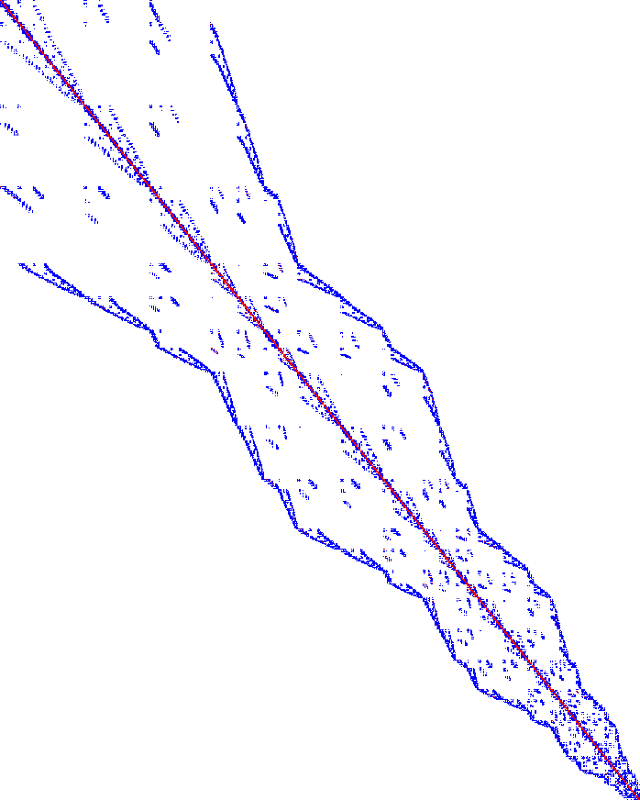
\includegraphics[width=1.15\textwidth]{figures/Dohp/EllipRCM}
    \end{column}
    \begin{column}{0.6\textwidth}
      \begin{itemize}
      \item Matrix assembly
        \begin{itemize}
        \item integration/fluxes: FPU
        \item insertion: memory/branching
        \end{itemize}
      \item Preconditioner setup
        \begin{itemize}
        \item coarse level operators
        \item overlapping subdomains
        \item (incomplete) factorization
        \end{itemize}
      \item Preconditioner application
        \begin{itemize}
        \item triangular solves/relaxation: memory
        \item coarse levels: network latency
        \end{itemize}
      \item Matrix multiplication
        \begin{itemize}
        \item Sparse storage: memory
        \item Matrix-free: FPU
        \end{itemize}
      \item Globalization
      \end{itemize}
    \end{column}
  \end{columns}
\end{frame}

\begin{frame} %{CPU Architecture}
  \begin{columns}
    \begin{column}{0.5\textwidth}
      {\centering Intel Clowertown \\
      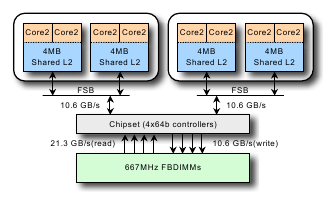
\includegraphics[width=\textwidth]{figures/hardware/IntelClovertown} }
    \begin{itemize}
    \item 75 Gflop/s
    \item 21 GB/s bandwidth
    \item thread + instruction level parallelism
    \item vector instructions (SSE)
    \end{itemize}
    \end{column}
    \begin{column}{0.5\textwidth}
      {\centering       AMD Opteron \\
      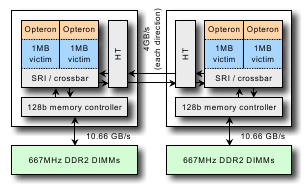
\includegraphics[width=\textwidth]{figures/hardware/AMDOpteron} }
    \begin{itemize}
    \item 17 Gflop/s
    \item 21 GB/s bandwidth
    \item thread + instruction level parallelism
    \item vector instructions (SSE)
    \end{itemize}
    \end{column}
  \end{columns}
\end{frame}

\begin{frame}{Hardware capabilities}
  \begin{columns}
    \begin{column}{0.5\textwidth}
      \begin{block}{Floating point unit}
        Recent Intel: each core can issue
        \begin{itemize}
        \item 1 packed add (latency 3)
        \item 1 packed mult (latency 5)
        \item One can include an aligned read
        \item Out of Order execution
        \item Peak: 10 Gflop/s (\texttt{double})
        \end{itemize}
      \end{block}
    \end{column}
    \begin{column}{0.5\textwidth}
      \begin{block}{Memory}
        \begin{itemize}
        \item $\sim 250$ cycle latency
        \item 5.3 GB/s bandwidth
        \item 1 \texttt{double} load / 3.7 cycles
        \item Pay by the cache line (32/64 B)
        \item L2 cache: $\sim 10$ cycle latency
        \end{itemize}
      \end{block}
    \end{column}
  \end{columns}
  \begin{block}{}%<2>{\alert{\Large It's \textbf{all} about the memory hierarchy}}
    \centering
    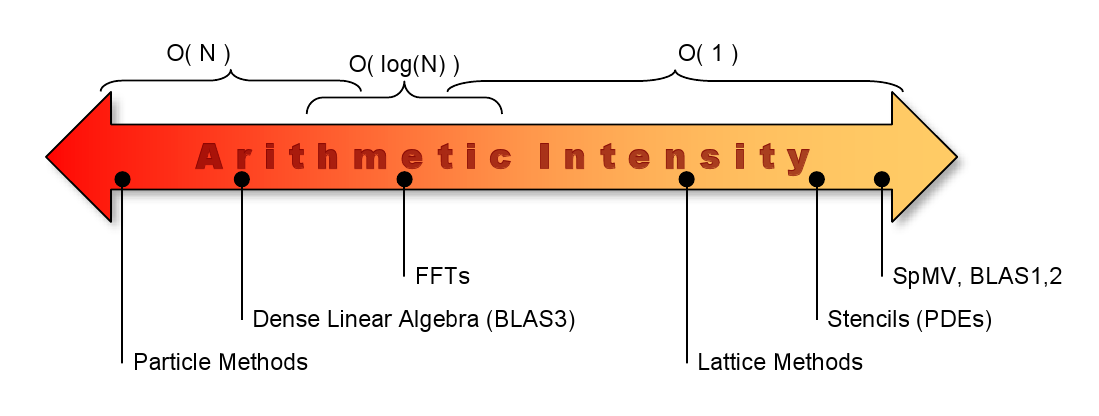
\includegraphics[width=0.85\textwidth]{figures/OlikerArithmeticIntensity} \\
    \vspace{-1em}
    {\tiny (Oliker et al. 2008)}
  \end{block}
\end{frame}

%\frame{
  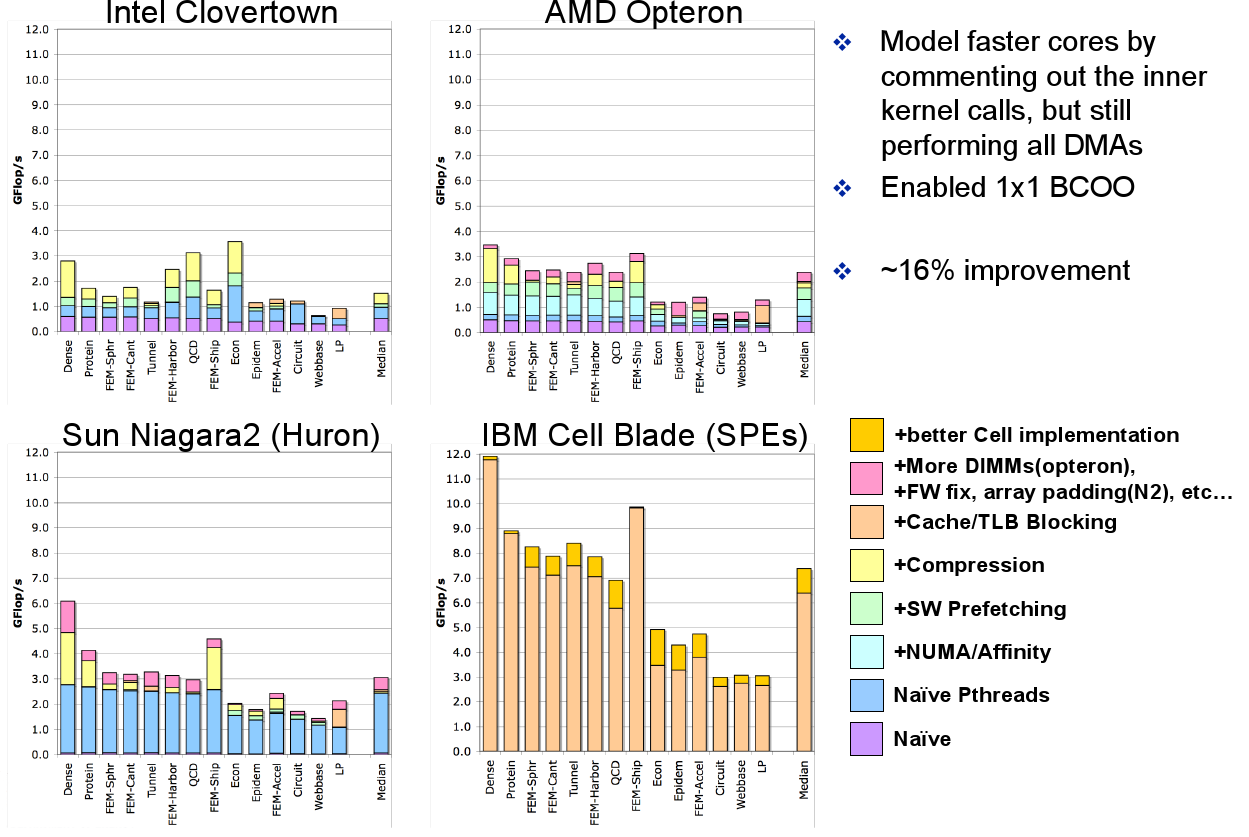
\includegraphics[width=\textwidth]{figures/OlikerSpMv} \\
  {\tiny (Oliker et al. \emph{Multi-core Optimization of Sparse Matrix Vector Multiplication}, 2008)}
}

\subsection{Sparse Matrix-Vector products}
\begin{frame}[fragile]{Sparse Mat-Vec performance model}
  \begin{block}{Compressed Sparse Row format (AIJ)}
    For $m \times n$ matrix with $N$ nonzeros
    \begin{itemize}
    \item[ai] row starts, length $m+1$
    \item[aj] column indices, length $N$, range $[0,n-1)$
    \item[aa] nonzero entries, length $N$, scalar values
    \end{itemize}
  \end{block}
\begin{columns}
\begin{column}{0.3\textwidth}
\[y \gets y + A x\]
\end{column}
\begin{column}{0.7\textwidth}
\begin{lstlisting}
  for (i=0; i<m; i++)
    for (j=ai[i]; j<ai[i+1]; j++)
      y[i] += aa[j] * x[aj[j]];
    \end{lstlisting}
  \end{column}
\end{columns}
  \begin{itemize}
  \item One add and one multiply per inner loop
  \item Scalar \code{aa[j]} and integer \code{aj[j]} only used once
  \item Must load \code{aj[j]} to read from \code{x}, may not reuse cache well
  \end{itemize}
\end{frame}

\begin{frame}[shrink=1]{Memory Bandwidth}
\begin{itemize}
\item Stream Triad benchmark (GB/s): $\bm w \gets \alpha \bm x + \bm y$
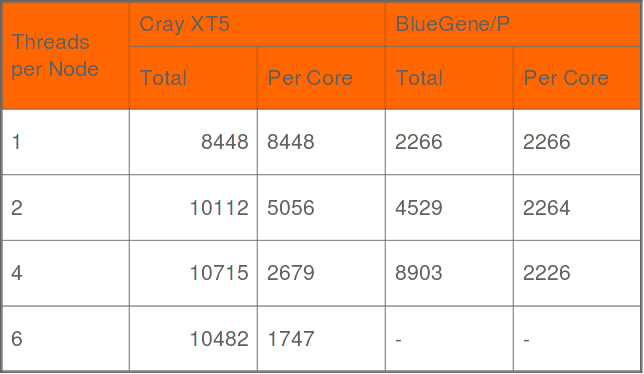
\includegraphics[width=0.8\textwidth]{figures/StreamTriadXT5VsBGP} \\
\item Sparse matrix-vector product: 6 bytes per flop
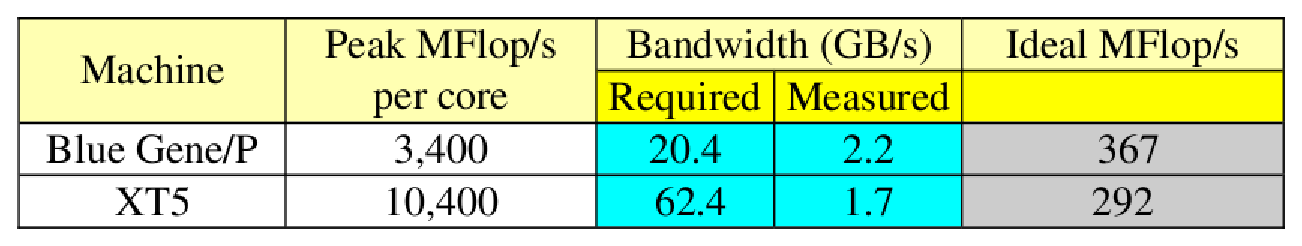
\includegraphics[width=0.8\textwidth]{figures/SparseMatVec} \\
%{\footnotesize (from Dinesh Kaushik)}
\end{itemize}
\end{frame}



\begin{frame}{Optimizing Sparse Mat-Vec}
  \begin{itemize}
  \item Order unknows so that vector reuses cache (Reverse Cuthill-McKee)
    \begin{itemize}
    \item Optimal: $\frac{(2 \text{ flops})(\text{bandwidth})}{\texttt{sizeof(Scalar)} + \texttt{sizeof(Int)}}$
    \item Usually improves strength of ILU and SOR
    \end{itemize}
  \item Coalesce indices for adjacent rows with same nonzero pattern (Inodes)
    \begin{itemize}
    \item Optimal: $\frac{(2 \text{ flops})(\text{bandwidth})}{\texttt{sizeof(Scalar)} + \texttt{sizeof(Int)}/i}$
    \item Can do block SOR (much stronger than scalar SOR)
    \item Default in PETSc, turn off with \code{-mat\_no\_inode}
    \item Requires ordering unknowns so that fields are interlaced, this
      is (much) better for memory use anyway
    \end{itemize}
  \item Use explicit blocking, hold one index per block (BAIJ format)
    \begin{itemize}
    \item Optimal: $\frac{(2 \text{ flops})(\text{bandwidth})}{\texttt{sizeof(Scalar)} + \texttt{sizeof(Int)}/b^2}$
    \item Block SOR and factorization
    \item Symbolic factorization works with blocks (much cheaper)
    \item Very regular memory access, unrolled dense kernels
    \item Faster insertion: \code{MatSetValuesBlocked()}
    \end{itemize}
  \end{itemize}
\end{frame}

\begin{frame}{Optimizing unassembled Mat-Vec}
  \begin{itemize}
  \item High order spatial discretizations do more work per node
    \begin{itemize}
    \item Dense tensor product kernel (like small BLAS3)
    \item Cubic ($Q_3$) elements in 3D can achieve $>60\%$ of peak FPU \\
      (compare to $< 6\%$ for assembled operators on multicore)
    \item Can store Jacobian information at quadrature points \\
      (usually pays off for $Q_2$ and higher in 3D)
    \item Spectral methods
    \item Often still need an assembled operator for preconditioning
    \end{itemize}
  \item Boundary element methods
    \begin{itemize}
    \item Dense kernels
    \item Fast Multipole Method (FMM)
    \end{itemize}
  \end{itemize}
\end{frame}

\subsection{Triangular solves}
\def\eps{.05}
\newcommand\lufactornodes[2]{
        \node [name=la] at (0,0.9) {};
        \node [name=da] at (0.1,0.9) {};
        \node [name=dau] at (0.1+#1,0.9+#2) {};
        \node [name=ua] at (1+#1,0.9+#2) {};
        \node [name=lb] at (0,0.7) {};
        \node [name=db] at (0.3,0.7) {};
        \node [name=dbu] at (0.3+#1,0.7+#2) {};
        \node [name=ub] at (1+#1,0.7+#2) {};
        \node [name=lc] at (0,0.5) {};
        \node [name=dc] at (0.5,0.5) {};
        \node [name=dcu] at (0.5+#1,0.5+#2) {};
        \node [name=uc] at (1+#1,0.5+#2) {};
        \node [name=ld] at (0,0.3) {};
        \node [name=dd] at (0.7,0.3) {};
        \node [name=ddu] at (0.7+#1,0.3+#2) {};
        \node [name=ud] at (1+#1,0.3+#2) {};
        \node [name=le] at (0,0.1) {};
        \node [name=de] at (0.9,0.1) {};
        \node [name=deu] at (0.9+#1,0.1+#2) {};
        \node [name=ue] at (1+#1,0.1+#2) {};
}
\newcommand\lufactors{
        \begin{scope}[color=red!90, ->]
          \draw [memread] (la) -- (da);
          \draw [memskip forward] (la) to[->,in=180] (da) to[in=135] (lb);
          \draw [memread] (lb) -- (db);
          \draw [memskip forward] (db) to (lc);
          \draw [memread] (lc) -- (dc);
          \draw [memskip forward] (dc) to (ld);
          \draw [memread] (ld) -- (dd);
          \draw [memskip forward] (dd) to (le);
          \draw [memread] (le) -- (de);
        \end{scope}
        \begin{scope}[color=blue!90, ->]
          \draw [memread] (ue) to (deu);
          \draw [memskip back] (ue) to[in=0] (deu) to[in=-45] (ud);
          \draw [memread] (ud) to (ddu);
          \draw [memskip back] (ddu) to (uc);
          \draw [memread] (uc) to (dcu);
          \draw [memskip back] (dcu) to (ub);
          \draw [memread] (ub) to (dbu);
          \draw [memskip back] (dbu) to (ua);
          \draw [memread] (ua) to (dau);
        \end{scope}
}

\begin{frame}{Storing Factors}
  \begin{columns}
    \begin{column}{0.3\textwidth}
      \begin{tikzpicture}[scale=3,
        memread/.style={line width=.5ex, >=to},
        memskip forward/.style={line width=.1ex, out=-90, in=135, >=latex},
        memskip back/.style={line width=.1ex, out=90, in=-45, >=latex}
        ]
        \shade [top color=red!4, bottom color=red!50] (0,1) -- (1,0) -- (0,0) -- cycle;
        \shade [top color=blue!4, bottom color=blue!50] (0,1) -- (1,0) -- (1,1) -- cycle;
        \lufactornodes{0}{0}
        \lufactors
        \node [anchor=south west, color=black] at (0,0) {\Huge $L$};
        \node [anchor=north east, color=black] at (1,1) {\Huge $U$};
      \end{tikzpicture}
    \end{column}
    \begin{column}{0.7\textwidth}
      \begin{itemize}
      \item Forward and back solves skip over unused part of each row
        \begin{itemize}
        \item Pollutes cache and bus with unused part, software prefetch helps some
        \end{itemize}
      \item Back solves move backward through memory and so does vector
        \begin{itemize}
        \item Core 2: hardware prefetch 16 forward-moving pointers and 4 backward-moving \\
          not across 4 KiB page boundaries
        \end{itemize}
      \end{itemize}
    \end{column}
  \end{columns}
  \begin{columns}
    \begin{column}{0.3\textwidth}
      \begin{tikzpicture}[scale=3,
        memread/.style={line width=.5ex, >=to},
        memskip forward/.style={line width=.1ex, out=-90, in=135, >=latex},
        memskip back/.style={line width=.1ex, out=90, in=-45, >=latex}
        ]
        \shade [top color=red!4, bottom color=red!50] (0,1) -- (1,0) -- (0,0) -- cycle;
        \shade [top color=blue!50, bottom color=blue!4] (0.05,1.05) -- (1.05,0.05) -- (1.05,1.05) -- cycle;
        \lufactornodes{.05}{.05}
        \lufactors
        \node [anchor=south west, color=black] at (0,0) {\Huge $L$};
        \node [anchor=north east, color=black] at (1,1) {\Huge $U$};
      \end{tikzpicture}
    \end{column}
    \begin{column}{0.7\textwidth}
      \begin{itemize}
      \item Forward and back solves get contiguous memory
      \item Move forward through memory for matrix entries
        \begin{itemize}
        \item Good for vector prefetch which necessarily tracks backward through memory
        \end{itemize}
      \end{itemize}
    \end{column}
  \end{columns}
\end{frame}

\begin{frame}{Improvement from better storage for factors}
  \begin{tabular}{|l|l|c|c|c|}
    \hline
    \multirow{2}{*}{Processor} & \multirow{2}{*}{Matrix} & SpMV & \multicolumn{2}{c|}{Triangular solves} \\
    & & (Mflop/s) & Old format & New format \\
    \hline
    \multirow{3}{*}{Core 2 Duo} & 7-point Laplace & 537 & 261 (49\%) & 447 (83\%) \\
               & 3D Euler AIJ & 620 & 260 (42\%) & 660 (106\%) \\
               & 3D Euler BAIJ & 890 & 468 (53\%) & 758 (85\%) \\
    \hline
    \multirow{3}{*}{BlueGene/P} & 7-point Laplace & 98 & 46 (47\%) & 62 (63\%) \\
               & 3D Euler AIJ & 148 & 99 (66\%) & 126 (85\%) \\
               & 3D Euler BAIJ & 303 & 198 (65\%) & 260 (86\%) \\
    \hline
  \end{tabular}
  \bigskip

  {\small Barry Smith and Hong Zhang, \emph{Sparse triangular solves for ILU revisited: \\
      data layout crucial to better performance}, submitted to
    Intl. J. of High Performance Computing Applications.}
\end{frame}


\section{Time Integration}
\subsection{Differential Algebraic Equations}
\begin{frame}{Stiff integrators}
  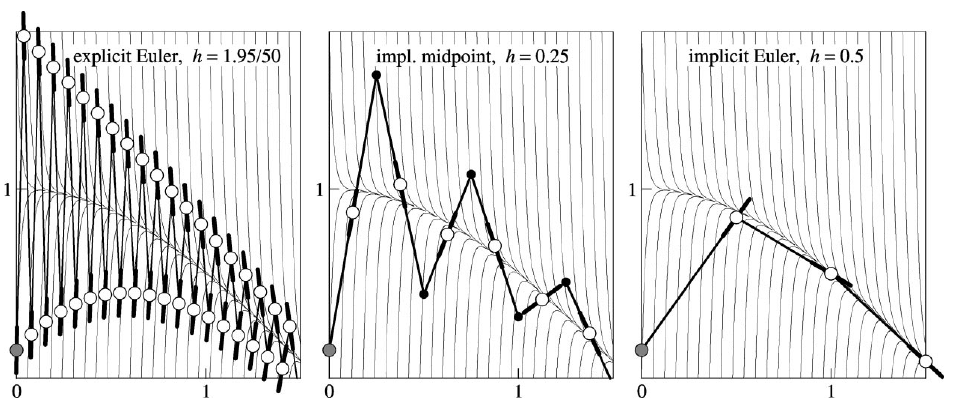
\includegraphics[width=\textwidth]{figures/HairerWanner-stiff}
  \vspace{-.9em}
  {\scriptsize \raggedleft (Hairer and Wanner, 1999)}
  \begin{equation*}
    \dot{x} + 50 (x - \cos t) = 0
  \end{equation*}
  \vspace{-1em}
  \begin{columns}
    \begin{column}{0.4\textwidth}
      \begin{itemize}
      \item $ \dot{x} = \lambda x $
      \item $\Rz(h \lambda) = x^{n+1}/x^n$
      \end{itemize}
    \end{column}
    \begin{column}{0.6\textwidth}
      \begin{itemize}
      \item $A$-stable: $\abs{\Rz(\{\Re [z] \le 0\})} \le 1$
      \item $L$-stable: $\lim_{z \to \infty} \Rz(z) = 0$
      \end{itemize}
    \end{column}
  \end{columns}
\end{frame}

\begin{frame}{Barriers}
  \begin{block}{Dahlquist's second barrier}
    An $A$-stable linear multistep method has order $p \le 2$.
  \end{block}
  \begin{block}{Diagonally implicit Runge-Kutta}
    A DIRK evaluates the first stage to order $q = 1$.
  \end{block}
  \begin{block}{Circumvent with general linear methods}
    \begin{equation*}
      \begin{bmatrix} Y \\ X^{n+1} \end{bmatrix}
      =
      \begin{bmatrix} A & U \\ B & V \end{bmatrix}
      \begin{bmatrix} h \dot{Y} \\ X^{n} \end{bmatrix}
    \end{equation*}
    \begin{itemize}
    \item stage values $Y = \{ y_1,\dotsc,y_s \}$
    \item Nordsieck vector passed between steps
      \[ X = \{x_1,\dotsc,x_r\} = \{x, h \dot{x}, h^2 \ddot{x}, \dotsc \} \]
    \item $A$ can be lower triangular (permits stages to be solved sequentially)
    \end{itemize}
  \end{block}
\end{frame}

\begin{frame}{Special class: IRKS (inherent Runge-Kutta stability)}
  \begin{itemize}
  \item $A$-stable
  \item $L$-stable
  \item order $p$, stage order $q$, $p=q=r-1=s-1$
  \item diagonally implicit
  \item Asymptotically correct error estimates for \\
    present method \emph{and} method of order $p+1$.
  \item Implemented in PETSc's TSGL (\code{-ts\_type gl})
    \begin{itemize}
    \item implicit DAE form: $f(t,x,\dot{x}) = 0$
    \item orders $p = 1,\dotsc,5$
    \item adaptive-order, adaptive-step controller
    \item plugin architecture for controllers
    \item make new methods available to the controller by giving their
      tableau, \\ error estimates computed automatically
    \item solve $f(t,x,x_0+\alpha x) = 0$ with SNES
    \end{itemize}
  \end{itemize}
  {\small Butcher, Jackiewicz, Wright, \emph{On error propagation in general linear methods for ordinary differential equations}, 2007.}
\end{frame}

\subsection{Strong stability preserving methods}
\begin{frame}{Strong stability preserving methods: \code{-ts\_type ssp}}
  \begin{itemize}
  \item Conservation laws $u_t + \divrg f(u) = 0$
  \item Discontinuous solutions, requires careful discretization \\
    to prevent spurious oscillations
  \item SSP property allows decoupling of spatial and time discretizations
  \item Choose spatial discretization that is stable with forward-Euler \\
    (e.g. TVD finite volume, ENO/WENO, Discontinuous Galerkin)
  \item Barriers for methods of order greater than 1 with $s$ stages
    \begin{equation*}
    c_{\text{eff}} = \frac{\abs{\lambda_{\text{max}}}\Delta t}{s\Delta x} <
    \begin{cases}
      1 & \text{Explicit}, \\
      2 & \text{Implicit}.
    \end{cases}
  \end{equation*}
  \item
    \begin{centering}
      \begin{tabular}{|l|c|l|c|c|}
        \hline
        Popular method & $c_{\text{eff}}$ & Improved method & $c_{\text{eff}}$ & Storage \\
        \hline
        SSPRK$(2,2)$ & 0.500 & SSPRK$(m,2)$ & $1-1/m$ & $2N^*$ \\
        SSPRK$(3,3)$ & 0.333 & SSPRK$(n^2,3)$ & $1-1/n$ & $2N$ \\
        SSPRK$(5,4)$ & 0.377 & SSPRK$(10,4)$ & $0.6$ & $2N$ \\
        \hline
      \end{tabular}
    \end{centering}
  \end{itemize}
  {\small David Ketcheson, \emph{Highly efficient strong stability-preserving Runge-Kutta methods with low-storage implementations}, 2008.}
\end{frame}


\section{Preconditioning using splitting methods}
\begin{frame}{Splitting for Multiphysics}
  \begin{equation*}
    \begin{bmatrix}
      A & B \\ C & D
    \end{bmatrix}
    \begin{bmatrix}
      x \\ y
    \end{bmatrix}
    =
    \begin{bmatrix}
      f \\ g
    \end{bmatrix}
  \end{equation*}
  \begin{itemize}\item Relaxation:
    \code{-pc\_fieldsplit\_type [additive,multiplicative,symmetric\_multiplicative]}
    \begin{equation*}
      \begin{bmatrix}
        A & \\  & D
      \end{bmatrix}^{-1} \qquad 
      \begin{bmatrix}
        A & \\ C & D
      \end{bmatrix}^{-1} \qquad
      \begin{bmatrix}
        A & \\  & \bm 1
      \end{bmatrix}^{-1}
      \left(
        \bm 1 -
        \begin{bmatrix}
          A & B \\ & \bm 1
        \end{bmatrix}
        \begin{bmatrix}
          A & \\ C & D
        \end{bmatrix}^{-1}
      \right)
    \end{equation*}
    \begin{itemize}
    \item Gauss-Seidel inspired, works when fields are loosely coupled
    \end{itemize}
  \item Factorization: \code{-pc\_fieldsplit\_type schur}
    \begin{align*}
      \begin{bmatrix}
        A & B \\ & S
      \end{bmatrix}^{-1}
      \begin{bmatrix}
        1 & \\ CA^{-1} & 1
      \end{bmatrix}^{-1}, \qquad
      S = D - C A^{-1} B
    \end{align*}
    \begin{itemize}
    \item robust (exact factorization), can often drop lower block
    \item how to precondition $S$ which is usually dense?
      \begin{itemize}
      \item interpret as differential operators, use approximate commutators
      \end{itemize}
    \end{itemize}
  \end{itemize}
\end{frame}

\begin{frame}{Examples of splitting for strong coupling}
  \begin{itemize}
  \item Incompressible flow
    \begin{gather*}
      J(u)
      \begin{bmatrix}
        w \\ p
      \end{bmatrix}
      \sim
      \begin{bmatrix}
        u\cdot\grad -\Delta & \grad \\
        -\divrg &  \\
      \end{bmatrix}
      \begin{bmatrix}
        w \\ p
      \end{bmatrix} \\
      S \sim \divrg (u\cdot\grad - \Delta)^{-1} \grad \approx \lap (u\cdot\grad - \Delta)^{-1}
    \end{gather*}
    \begin{itemize}
    \item $S^{-1}$ requires solve with a Laplacian and application of an
      advection-diffusion operator defined in pressure space (Elman et
      al, 2008)
    \end{itemize}
  \item Shallow water with stiff gravity wave, $\alpha = 1/\Delta t$, wave speed $\sqrt{gh}$
    \begin{gather*}
      J(h,uh)
      \begin{bmatrix} h' \\ uh' \end{bmatrix}
      \sim
      \begin{bmatrix}
        \alpha & \divrg \\
        g h \grad & \alpha
      \end{bmatrix}
      \begin{bmatrix} h' \\ uh' \end{bmatrix}
      + (\text{non-stiff terms})
      \\
      S \sim \alpha - \alpha^{-1} g \divrg h\grad
    \end{gather*}
    \begin{itemize}
    \item Scalar parabolic operator, good for multigrid \\
      (Mousseau, Knoll, and Reisner, 2002)
    \end{itemize}
  \end{itemize}
\end{frame}


\section{Hydrostatic Ice}
\begin{frame}[shrink=5]{Hydrostatic equations for ice sheet flow}
  \begin{itemize}
  \item Valid when $w_x \ll u_z$, independent of basal friction {\small (Schoof\&Hindmarsh 2010)}
  \item Eliminate $p$ and $w$ from Stokes by incompressibility:\\
    \quad 3D elliptic system for $\bm u = (u,v)$
    \begin{align*}
      - \nabla\cdot \left[ \eta
        \begin{pmatrix}
          4 u_x + 2 v_y & u_y + v_x & u_z \\
          u_y + v_x & 2 u_x + 4 v_y & v_z
        \end{pmatrix} \right] + \rho g \bar\nabla h & = 0
    \end{align*}
    \begin{align*}
      \eta(\theta,\gamma) &= \frac{B(\theta)}{2} (\gamma_0 + \gamma)^{\frac{1-\mathfrak n}{2\mathfrak n}}, \qquad \mathfrak n \approx 3 \\
      \gamma &= u_x^2 + v_y^2 + u_xv_y + \frac 1 4 (u_y+v_x)^2 + \frac 1 4 u_z^2 + \frac 1 4 v_z^2
    \end{align*}
    and slip boundary $\sigma \cdot \bm n = \beta^2 \bm u$ where
    \begin{align*}
      \beta^2(\gamma_b) &= \beta_0^2 (\epsilon_b^2 + \gamma_b)^{\frac{\mathfrak m-1}{2}}, \qquad 0 < \mathfrak m \le 1 \\
      \gamma_b &= \frac 1 2 (u^2 + v^2)
    \end{align*}
  \item $Q_1$ FEM with Newton-Krylov-Multigrid solver in PETSc: \code{src/snes/examples/tutorials/ex48.c}
  \end{itemize}
\end{frame}

\frame{
  \vspace{-8em}
  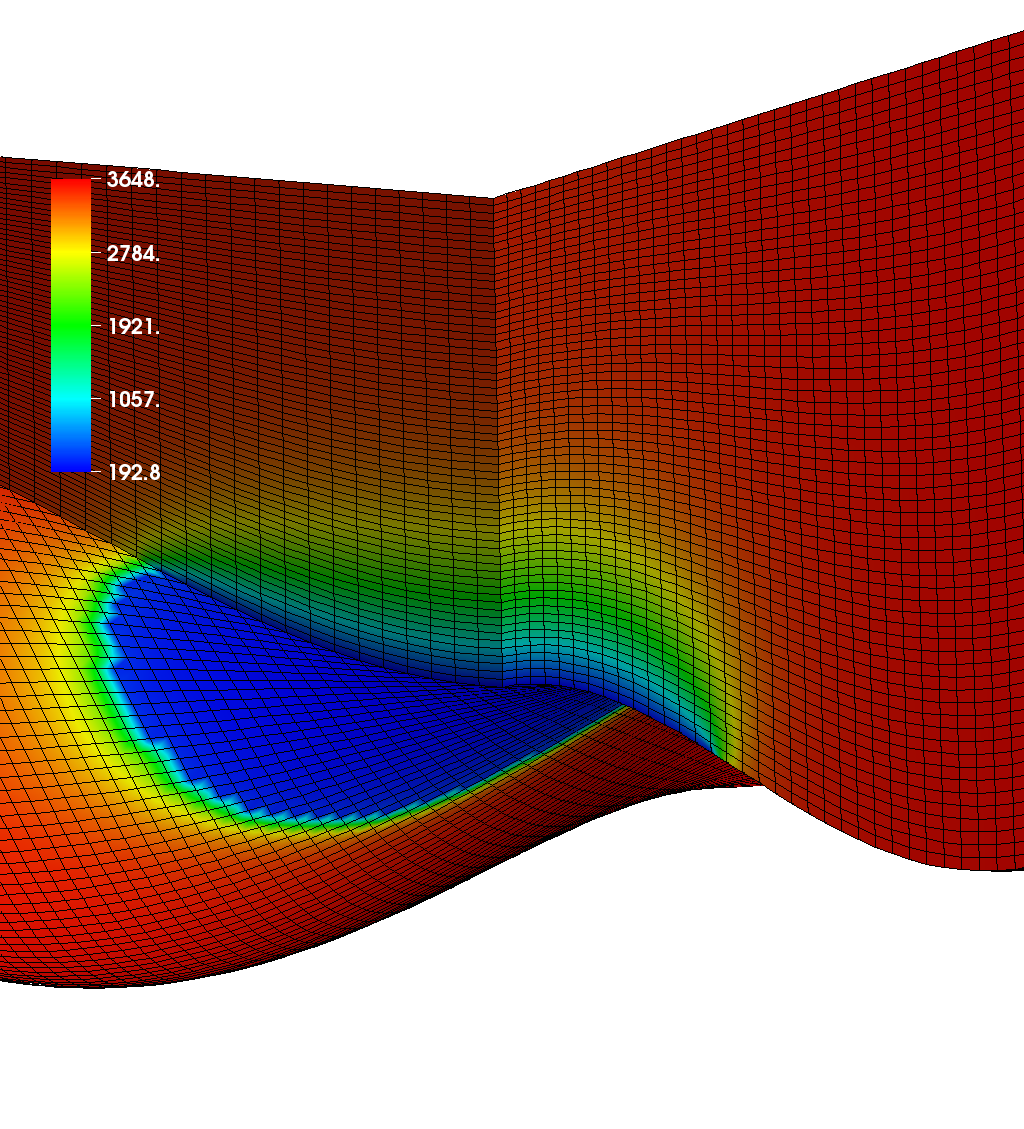
\includegraphics[width=1.2\textwidth]{figures/THI/x-5km-m8p5l5-clip}
}

\begin{frame}{What about splitting at the global level?}
  \begin{itemize}\footnotesize
  \item Split $(u,v)$ multiplicatively at global level: {\code{\small -pc\_type fieldsplit}}
    \begin{itemize} 
    \item parallel direct solve in splits \\
      {\code{-fieldsplit\_pc\_type cholesky -fieldsplit\_pc\_factor\_mat\_solver\_package mumps}}
    \item Split additively instead \\
      {\code{-pc\_fieldsplit\_type additive}}
    \item Parallel ML in splits, ASM(1)/ICC(1) on levels \\
      {\code{-fieldsplit\_pc\_type asm \\ \qquad -fieldsplit\_sub\_pc\_type icc \\ \qquad -fieldsplit\_sub\_pc\_factor\_levels 1}}
    \item Parallel BoomerAMG in splits \\
      {\code{-fieldsplit\_pc\_type hypre}}
    \item ASM/Cholesky in splits \\
      {\code{-fieldsplit\_pc\_type asm \\ \qquad -fieldsplit\_sub\_pc\_type cholesky}}
    \item ASM/ICC(0) in splits \\
      {\code{-fieldsplit\_pc\_type asm \\ \qquad -fieldsplit\_sub\_pc\_type icc}}
    \end{itemize}
  \end{itemize}
\end{frame}

\begin{frame}{Split in subdomains?}
  \begin{itemize}
  \item ASM on coupled system: {\code{-pc\_type asm}}
    \begin{itemize}
    \item Split in subdomains, Cholesky in splits \\
    {\code{-sub\_pc\_type fieldsplit \\ \qquad -sub\_fieldsplit\_pc\_type cholesky}}
    \item Split in subdomainst, ML in splits \\
      {\code{-sub\_pc\_type fieldsplit \\ \qquad -sub\_fieldsplit\_pc\_type ml}}
    \item Split in subdomains, BoomerAMG in splits \\
      {\code{-sub\_pc\_type fieldsplit \\ \qquad -sub\_fieldsplit\_pc\_type hypre}}
    \item Split in subdomains, ICC(1) in splits \\
      {\code{-sub\_pc\_type fieldsplit \\ \qquad -sub\_fieldsplit\_pc\_type icc}}
    \item Block ICC(0) on subdomains (no splitting), stored as block symmetric
      {\code{-sub\_pc\_type icc -da\_mat\_type sbaij}}
    \end{itemize}
  \end{itemize}
\end{frame}

\begin{frame}{Coupled Multigrids}
  \begin{itemize}
  \item Geometric multigrid with isotropic coarsening, ASM(1)/Cholesky and ASM(0)/ICC(0) on levels \\
    {\code{\small -mg\_levels\_pc\_type bjacobi -mg\_levels\_sub\_pc\_type icc -mg\_levels\_1\_pc\_type asm -mg\_levels\_1\_sub\_pc\_type cholesky}}
  \item \ldots with Galerkin coarse operators \\
    {\code{\small -pc\_mg\_galerkin}}
  \item \ldots with ML's aggregates \\
    {\code{\small -pc\_type ml -mg\_levels\_pc\_type asm}}
  \item Geometric multigrid with aggressive semi-coarsening, ASM(1)/Cholesky and ASM(0)/ICC(0) on levels \\
    {\code{\small -da\_refine\_hierarchy\_x 1,1,8,8 -da\_refine\_hierarchy\_y 2,2,1,1 -da\_refine\_hierarachy\_z 2,2,1,1}}
  \item Simulate 1024 cores, interactively, on my laptop \\
    {\code{\small -mg\_levels\_pc\_asm\_blocks 1024}}
  \end{itemize}
\end{frame}

\begin{frame}{Summary of solvers}
  \centering
  \begin{tabular}{|l|c|}
    \hline
    Method & Avg Krylov/Newton \\
    \hline
    Global multiplicative FieldSplit, ASM/LU & 175 \\
    Global multiplicative FieldSplit, BoomerAMG & 59 \\
    Global multiplicative FieldSplit, strong ML & 71 \\
    Global additive FieldSplit, ASM/LU & 197 \\
    Global ASM, FieldSplit/LU inside & 215 \\
    Global ASM, LU inside & 167 \\
    Coupled BoomerAMG & 60 \\
    Coupled ML with strong smoothers & 72 \\
    Geometric multigrid & 11 \\
    Geometric multigrid, Galerkin coarse & 122 \\
    \hline
  \end{tabular} \\
  {Smallish size $40\times 40\times 10$, relatively extreme parameters}
\end{frame}

\begin{frame}{Linear solve performance}
  \centering
  \includegraphics[width=\textwidth]{figures/THI/linear4}
\end{frame}

\begin{frame}{Status-quo Picard}
  \includegraphics[width=\textwidth]{figures/THI/z-picard-mult-noseq}
\end{frame}

\begin{frame}{Grid sequencing: \code{-dmmg\_grid\_sequence}}
    \includegraphics[width=0.9\textwidth]{figures/THI/z-mult-o1-r2}
\end{frame}

\begin{frame}{Avoid oversolving}
    \includegraphics[width=0.9\textwidth]{figures/THI/z-mult-o1-ew} \\
    Luis Chacon's variant of Eisenstat-Walker: \\
    \code{\footnotesize -snes\_ksp\_ew -snes\_ksp\_ew\_rtolmax 0.5 -snes\_ksp\_ew\_version 3}
\end{frame}


\begin{frame}{Thoughts on Multigrid}
  \begin{itemize}
  \item Rapid coarsening is essential for weak scalability
    \begin{itemize}
    \item Push the algorithm towards ``multilevel domain decomposition''
    \end{itemize}
  \item Energy minimizing interpolants (Wan, Chan, and Smith 2000)
    \begin{itemize}
    \item Similar to exotic Schwarz methods, see Dohrmann and Widlund 2008, 2009
    \item Closely related to FETI-DP/BDDC coarse spaces
    \end{itemize}
  \item (Precondition with) first-order upwind for transport/waves
  \item Smooth all components together (block SOR, Vanka smoothers for indefinite problems)
  \item Interpolation operators must be compatible with physics (e.g. inf-sup conditions)
  \item Ordering of unknowns can make incomplete factorization behave \\
    similar to line smoothers
  \item Nonlinear multigrid (FAS) is worth trying if pointwise or block \\
    residuals are cheap, or globalization is especially challenging
  \item Monotone multigrid (Kornhuber) for variational inequalities
  \item Boundary conditions in subdomain problems (``optimized Schwarz'')
  \end{itemize}
\end{frame}


\begin{frame}{Wrap-up}
  \begin{itemize}
  \item PETSc can help you
    \begin{itemize}
    \item easily construct a code to experiment with ideas
    \item scale an existing code base
    \item incorporate more scalable or higher performance algorithms
    \item attain high performance on a variety of architectures
    \item debug and profile a parallel application (not discussed today)
    \item package and distribute your code (e.g. graph algorithms, \\
      domain decomposition and multilevel solvers), \code{-{}-download-xxx}
    \end{itemize}
  \item I will be around most of today, find me to discuss
    \begin{itemize}
    \item new and old features in PETSc
    \item performance, scalability, and algorithms
    \item design of new codes
    \item integration with your existing application
    \end{itemize}
  \item \url{http://mcs.anl.gov/petsc}
  \item \url{petsc-users@mcs.anl.gov} and \url{petsc-dev@mcs.anl.gov}
  \item \url{petsc-maint@mcs.anl.gov}
  \end{itemize}
\end{frame}

\end{document}
